\documentclass[tikz,border=1mm]{standalone}
\usepackage{amssymb}
\usetikzlibrary{matrix,chains,positioning,decorations.pathreplacing,arrows,shapes.geometric}

% Code modified from here https://tex.stackexchange.com/questions/505741/architecture-neural-network-with-weights

\begin{document}
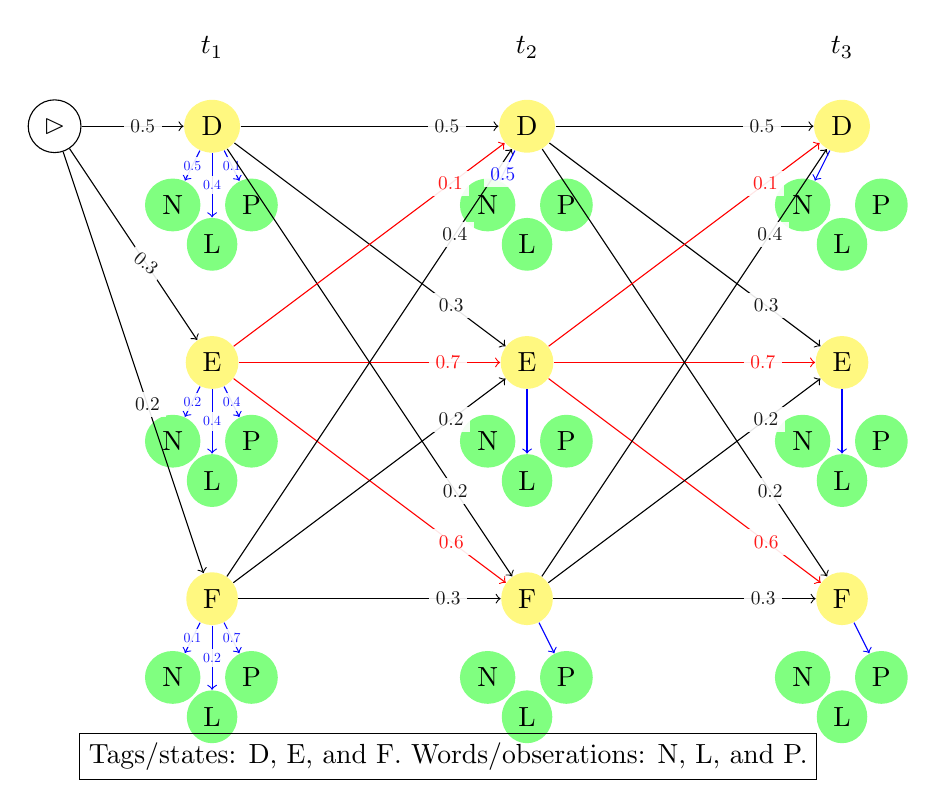
\begin{tikzpicture}%[>=latex]

% Step 1 
\path
(0,0)         node[circle,draw,align=center] (origin) {$\rhd$} 
+(2,1)     node  (t1) {$t_1$}
+(2,0)     node[ellipse,fill=yellow!50]  (t11) {D} % {$t_{1,1}$}
% +(2,-1)     node[ellipse,fill=green!50]  (w11) {N, L, P, C, S}
+(1.5,-1)     node[ellipse,fill=green!50]  (w11N) {N}
+(2,-1.5)     node[ellipse,fill=green!50]  (w11L) {L}
+(2.5,-1)     node[ellipse,fill=green!50]  (w11P) {P}
+(2,-3)     node[ellipse,fill=yellow!50]  (t12) {E} % {$t_{1,2}$}
% +(2,-4)     node[ellipse,fill=green!50]  (w12) {N, L, P, C, S}
+(1.5,-4)     node[ellipse,fill=green!50]  (w12N) {N}
+(2,-4.5)     node[ellipse,fill=green!50]  (w12L) {L}
+(2.5,-4)     node[ellipse,fill=green!50]  (w12P) {P}
+(2,-6)     node[ellipse,fill=yellow!50]  (t13) {F} % {$t_{1,3}$}
% +(2,-7)     node[ellipse,fill=green!50]  (w13) {N, L, P, C, S}
+(1.5,-7)     node[ellipse,fill=green!50]  (w13N) {N}
+(2,-7.5)     node[ellipse,fill=green!50]  (w13L) {L}
+(2.5,-7)     node[ellipse,fill=green!50]  (w13P) {P}
;

\draw[->, black] (origin)--(t11) node[pos=.6, fill=white, opacity=.9, scale=0.7]{$0.5$};
\draw[->, black] (origin)--(t12) node[pos=.6, fill=white, opacity=.9, scale=0.7, rotate=320]{$0.3$};
\draw[->, black] (origin)--(t13) node[pos=.6, fill=white, opacity=.9, scale=0.7]{$0.2$};
\draw[->, blue] (t11)--(w11N)  node[pos=.5, fill=white, opacity=.9, scale=0.5]{$0.5$};
\draw[->, blue] (t11)--(w11L)  node[pos=.5, fill=white, opacity=.9, scale=0.5]{$0.4$};
\draw[->, blue] (t11)--(w11P)  node[pos=.5, fill=white, opacity=.9, scale=0.5]{$0.1$};
\draw[->, blue] (t12)--(w12N)  node[pos=.5, fill=white, opacity=.9, scale=0.5]{$0.2$};
\draw[->, blue] (t12)--(w12L)  node[pos=.5, fill=white, opacity=.9, scale=0.5]{$0.4$};
\draw[->, blue] (t12)--(w12P)  node[pos=.5, fill=white, opacity=.9, scale=0.5]{$0.4$};
\draw[->, blue] (t13)--(w13N)  node[pos=.5, fill=white, opacity=.9, scale=0.5]{$0.1$};
\draw[->, blue] (t13)--(w13L)  node[pos=.5, fill=white, opacity=.9, scale=0.5]{$0.2$};
\draw[->, blue] (t13)--(w13P)  node[pos=.5, fill=white, opacity=.9, scale=0.5]{$0.7$};


% End step 1 



% Step 2 
\path 
+(6,1)     node  (t2) {$t_2$}
+(6,0)     node[ellipse,fill=yellow!50]  (t21) {D} % {$t_{1,1}$}
% +(2,-1)     node[ellipse,fill=green!50]  (w11) {N, L, P, C, S}
+(5.5,-1)     node[ellipse,fill=green!50]  (w21N) {N}
+(6,-1.5)     node[ellipse,fill=green!50]  (w21L) {L}
+(6.5,-1)     node[ellipse,fill=green!50]  (w21P) {P}
+(6,-3)     node[ellipse,fill=yellow!50]  (t22) {E} % {$t_{1,2}$}
% +(2,-4)     node[ellipse,fill=green!50]  (w12) {N, L, P, C, S}
+(5.5,-4)     node[ellipse,fill=green!50]  (w22N) {N}
+(6,-4.5)     node[ellipse,fill=green!50]  (w22L) {L}
+(6.5,-4)     node[ellipse,fill=green!50]  (w22P) {P}
+(6,-6)     node[ellipse,fill=yellow!50]  (t23) {F} % {$t_{1,3}$}
% +(2,-7)     node[ellipse,fill=green!50]  (w13) {N, L, P, C, S}
+(5.5,-7)     node[ellipse,fill=green!50]  (w23N) {N}
+(6,-7.5)     node[ellipse,fill=green!50]  (w23L) {L}
+(6.5,-7)     node[ellipse,fill=green!50]  (w23P) {P}
;

\draw[->, black] (t11)--(t21) node[pos=.8, fill=white, opacity=.9, scale=0.7]{$0.5$};
\draw[->, black] (t11)--(t22) node[pos=.8, fill=white, opacity=.9, scale=0.7]{$0.3$};
\draw[->, black] (t11)--(t23) node[pos=.8, fill=white, opacity=.9, scale=0.7]{$0.2$};

\draw[->, red] (t12)--(t21) node[pos=.8, fill=white, opacity=.9, scale=0.7]{$0.1$};
\draw[->, red] (t12)--(t22) node[pos=.8, fill=white, opacity=.9, scale=0.7]{$0.7$};
\draw[->, red] (t12)--(t23) node[pos=.8, fill=white, opacity=.9, scale=0.7]{$0.6$};

\draw[->, black] (t13)--(t21) node[pos=.8, fill=white, opacity=.9, scale=0.7]{$0.4$};
\draw[->, black] (t13)--(t22) node[pos=.8, fill=white, opacity=.9, scale=0.7]{$0.2$};
\draw[->, black] (t13)--(t23) node[pos=.8, fill=white, opacity=.9, scale=0.7]{$0.3$};

\draw[->, blue] (t21)--(w21N) node[pos=.8, fill=white, opacity=.9, scale=0.7]{$0.5$};;
\draw[->, blue] (t22)--(w22L) ;
\draw[->, blue] (t23)--(w23P) ;

% step 3: 
\path 
+(2+8,1)     node  (t3) {$t_3$}
+(2+8,0)     node[ellipse,fill=yellow!50]  (t31) {D} % {$t_{1,1}$}
% +(2,-1)     node[ellipse,fill=green!50]  (w11) {N, L, P, C, S}
+(1.5+8,-1)     node[ellipse,fill=green!50]  (w31N) {N}
+(2+8,-1.5)     node[ellipse,fill=green!50]  (w31L) {L}
+(2.5+8,-1)     node[ellipse,fill=green!50]  (w31P) {P}
+(2+8,-3)     node[ellipse,fill=yellow!50]  (t32) {E} % {$t_{1,2}$}
% +(2,-4)     node[ellipse,fill=green!50]  (w12) {N, L, P, C, S}
+(1.5+8,-4)     node[ellipse,fill=green!50]  (w32N) {N}
+(2+8,-4.5)     node[ellipse,fill=green!50]  (w32L) {L}
+(2.5+8,-4)     node[ellipse,fill=green!50]  (w32P) {P}
+(2+8,-6)     node[ellipse,fill=yellow!50]  (t33) {F} % {$t_{1,3}$}
% +(2,-7)     node[ellipse,fill=green!50]  (w13) {N, L, P, C, S}
+(1.5+8,-7)     node[ellipse,fill=green!50]  (w33N) {N}
+(2+8,-7.5)     node[ellipse,fill=green!50]  (w33L) {L}
+(2.5+8,-7)     node[ellipse,fill=green!50]  (w33P) {P}
;

\draw[->, black] (t21)--(t31) node[pos=.8, fill=white, opacity=.9, scale=0.7]{$0.5$};
\draw[->, black] (t21)--(t32) node[pos=.8, fill=white, opacity=.9, scale=0.7]{$0.3$};
\draw[->, black] (t21)--(t33) node[pos=.8, fill=white, opacity=.9, scale=0.7]{$0.2$};

\draw[->, red] (t22)--(t31) node[pos=.8, fill=white, opacity=.9, scale=0.7]{$0.1$};
\draw[->, red] (t22)--(t32) node[pos=.8, fill=white, opacity=.9, scale=0.7]{$0.7$};
\draw[->, red] (t22)--(t33) node[pos=.8, fill=white, opacity=.9, scale=0.7]{$0.6$};

\draw[->, black] (t23)--(t31) node[pos=.8, fill=white, opacity=.9, scale=0.7]{$0.4$};
\draw[->, black] (t23)--(t32) node[pos=.8, fill=white, opacity=.9, scale=0.7]{$0.2$};
\draw[->, black] (t23)--(t33) node[pos=.8, fill=white, opacity=.9, scale=0.7]{$0.3$};

\draw[->, blue] (t31)--(w31N) ;
\draw[->, blue] (t32)--(w32L) ;
\draw[->, blue] (t33)--(w33P) ;

\node[draw] at (5,-8) {Tags/states: D, E, and F. Words/obserations: N, L, and P.};

\end{tikzpicture}
\end{document}
